\documentclass[10pt,landscape]{article}
\usepackage{multicol}
\usepackage{calc}
\usepackage{ifthen}
\usepackage[landscape]{geometry}
\usepackage{hyperref}
\usepackage{graphicx}
\usepackage{amsmath}
\usepackage{tikz}
\usetikzlibrary{shapes.geometric, arrows}
\usepackage[table]{xcolor}
% To make this come out properly in landscape mode, do one of the following
% 1.
%  pdflatex latexsheet.tex
%
% 2.
%  latex latexsheet.tex
%  dvips -P pdf  -t landscape latexsheet.dvi
%  ps2pdf latexsheet.ps


% If you're reading this, be prepared for confusion.  Making this was
% a learning experience for me, and it shows.  Much of the placement
% was hacked in; if you make it better, let me know...


% 2008-04
% Changed page margin code to use the geometry package. Also added code for
% conditional page margins, depending on paper size. Thanks to Uwe Ziegenhagen
% for the suggestions.

% 2006-08
% Made changes based on suggestions from Gene Cooperman. <gene at ccs.neu.edu>


% To Do:
% \listoffigures \listoftables
% \setcounter{secnumdepth}{0}


% This sets page margins to .5 inch if using letter paper, and to 1cm
% if using A4 paper. (This probably isn't strictly necessary.)
% If using another size paper, use default 1cm margins.
\ifthenelse{\lengthtest { \paperwidth = 11in}}
	{ \geometry{top=.5in,left=.5in,right=.5in,bottom=.5in} }
	{\ifthenelse{ \lengthtest{ \paperwidth = 297mm}}
		{\geometry{top=1cm,left=1cm,right=1cm,bottom=1cm} }
		{\geometry{top=1cm,left=1cm,right=1cm,bottom=1cm} }
	}
% Turn off header and footer
\pagestyle{empty}
 

% Redefine section commands to use less space
\makeatletter
\renewcommand{\section}{\@startsection{section}{1}{0mm}%
                                {-1ex plus -.5ex minus -.2ex}%
                                {0.5ex plus .2ex}%x
                                {\normalfont\large\bfseries}}
\renewcommand{\subsection}{\@startsection{subsection}{2}{0mm}%
                                {-1explus -.5ex minus -.2ex}%
                                {0.5ex plus .2ex}%
                                {\normalfont\normalsize\bfseries}}
\renewcommand{\subsubsection}{\@startsection{subsubsection}{3}{0mm}%
                                {-1ex plus -.5ex minus -.2ex}%
                                {1ex plus .2ex}%
                                {\normalfont\small\bfseries}}
\makeatother

% Define BibTeX command
\def\BibTeX{{\rm B\kern-.05em{\sc i\kern-.025em b}\kern-.08em
    T\kern-.1667em\lower.7ex\hbox{E}\kern-.125emX}}

% Don't print section numbers
\setcounter{secnumdepth}{0}


\setlength{\parindent}{0pt}
\setlength{\parskip}{0pt plus 0.5ex}


% -----------------------------------------------------------------------

\begin{document}

\raggedright
\footnotesize
\begin{multicols}{3}


% multicol parameters
% These lengths are set only within the two main columns
%\setlength{\columnseprule}{0.25pt}
\setlength{\premulticols}{1pt}
\setlength{\postmulticols}{1pt}
\setlength{\multicolsep}{1pt}
\setlength{\columnsep}{2pt}

\hrule height 0.3mm
\section{HTTP - Application Protocol}
\begin{tabular}{p{0.40\linewidth}p{0.50\linewidth}}
\verb!non-persistent! & one object per TCP connection \\
\verb!persistent!  & multiple connection per TCP connection \\
\verb!pipelined persistent! & multiple requests, without blocking for responses, responses in order of requests \\
\verb!persistent out-of-order!  & multiple requests, responses can be in different order \\
\end{tabular}
\hrule height 0.3mm 
\section{DNS - Application Protocol}
\begin{itemize}
    \setlength{\itemsep}{0pt}
    \item \textbf{NS Record (Name Server Record)}  
    Specifies the authoritative name servers for a domain. In this case, the authoritative name servers for \texttt{tu-berlin.de} are
    \item \textbf{Authority Section}  
    Lists the authoritative name servers for the queried domain. These servers are responsible for providing the official DNS records. The TTL (Time To Live) for these records is 28,800 seconds.
    \item \textbf{Additional Section}  
    Provides extra information, such as the IP addresses of the authoritative name servers, to speed up resolution.  
\end{itemize}
\hrule
\begin{itemize}
\setlength{\itemsep}{0pt}
    \item \textbf{Recursive DNS:} The local DNS resolver does all the work and returns the final answer to the client.
    \item \textbf{Iterative DNS:} The resolver receives a referral and queries the next DNS server (root, TLD, authoritative) in the hierarchy.
    \item \textbf{Root DNS Servers:} There are 13 root servers worldwide, distributed via Anycast, responding from the closest instance.
    \item \textbf{Local DNS Queries:} Queries from clients to local resolvers are typically recursive.
    \item \textbf{Root and TLD Server Queries:} Queries to root and TLD servers are iterative, with referrals to the next server.
    \item \textbf{Authoritative Server Queries:} Queries to authoritative servers are also iterative, with the final answer provided (e.g., A record).
\end{itemize}
\vspace{0.1cm}
    \begin{minipage}{0.49\columnwidth}
    \begin{center}
    \textbf{Iterative}
      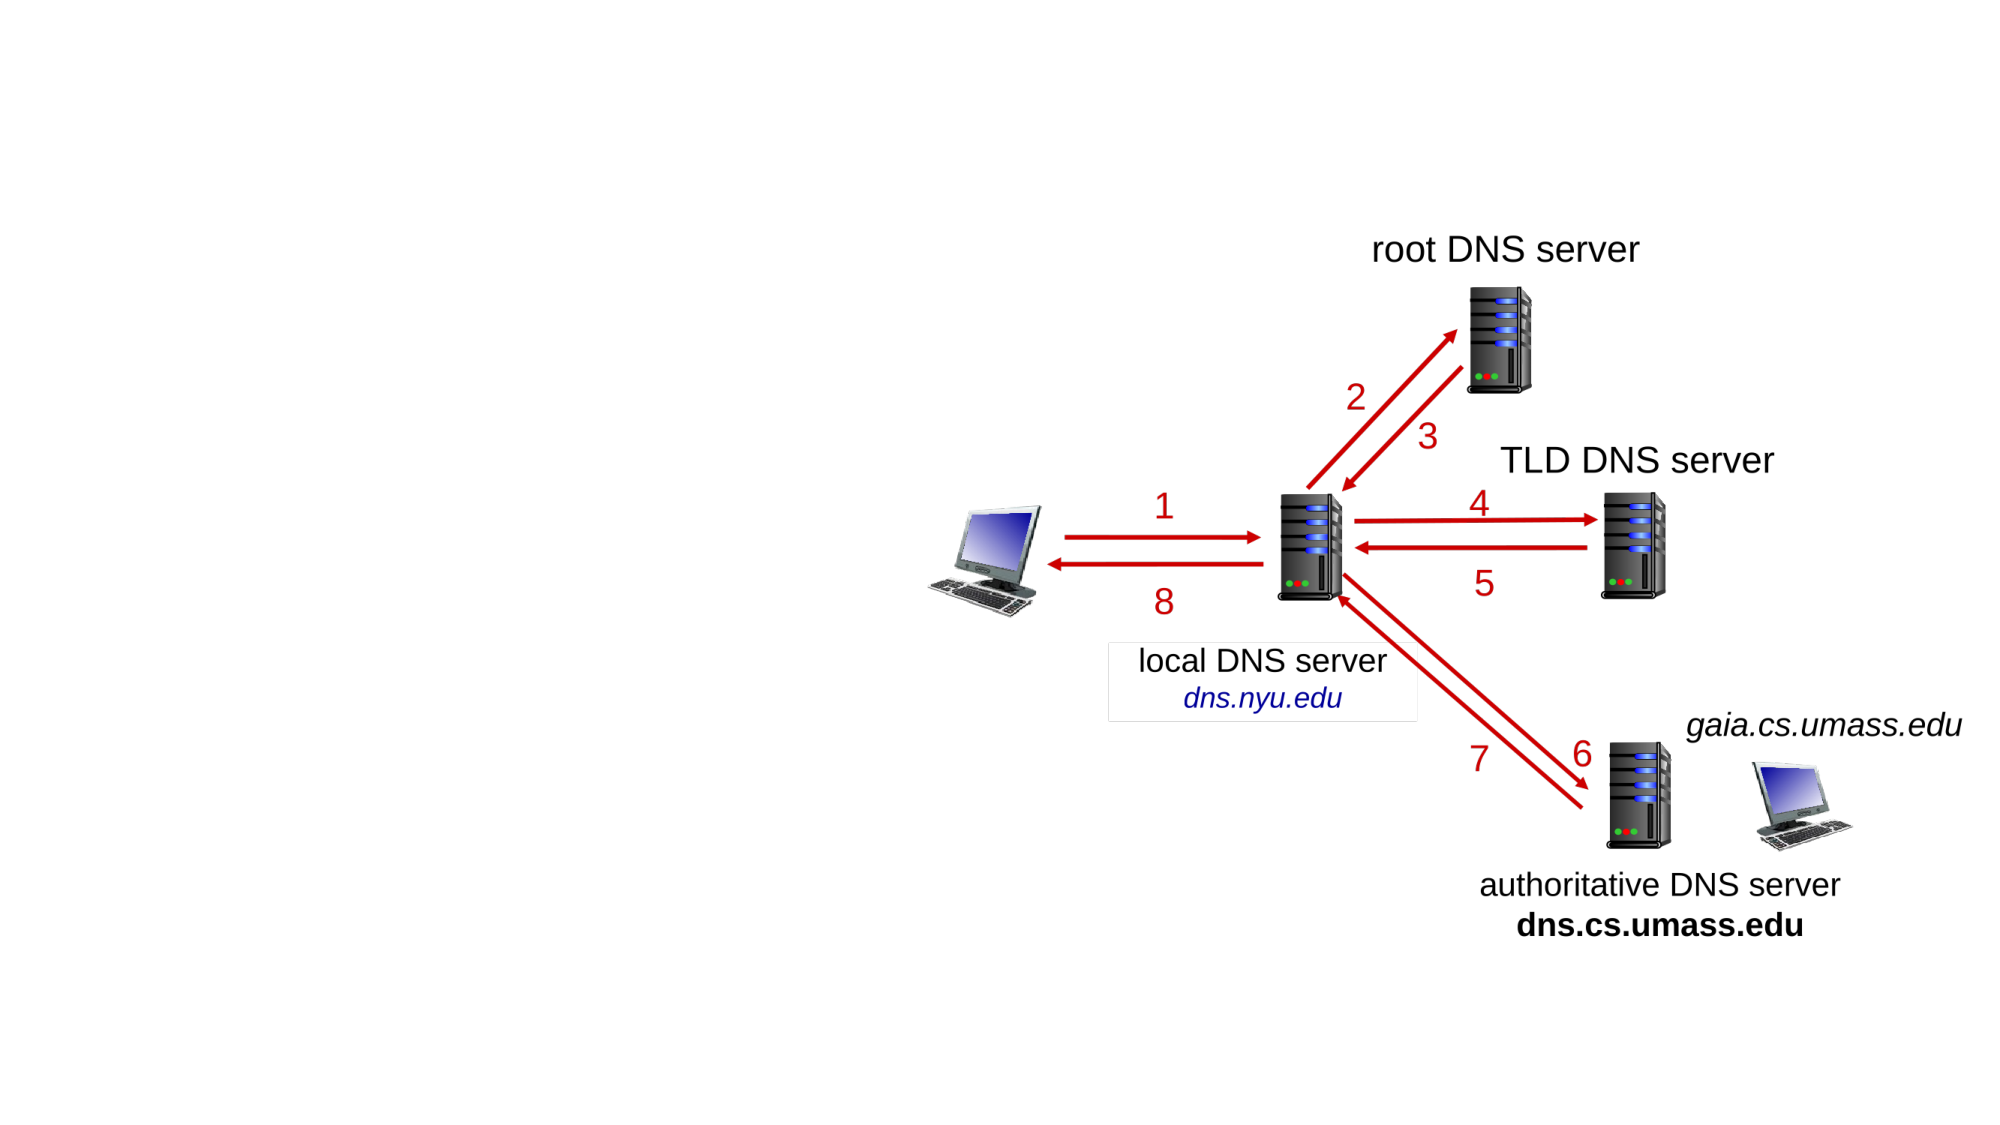
\includegraphics[width=4cm,trim={15cm 3cm 0 4cm},clip]{img/dns_iterated.pdf}  
    \end{center}
    \end{minipage}
    \begin{minipage}{0.49\columnwidth}
      \begin{center}
        \textbf{Recursive}
        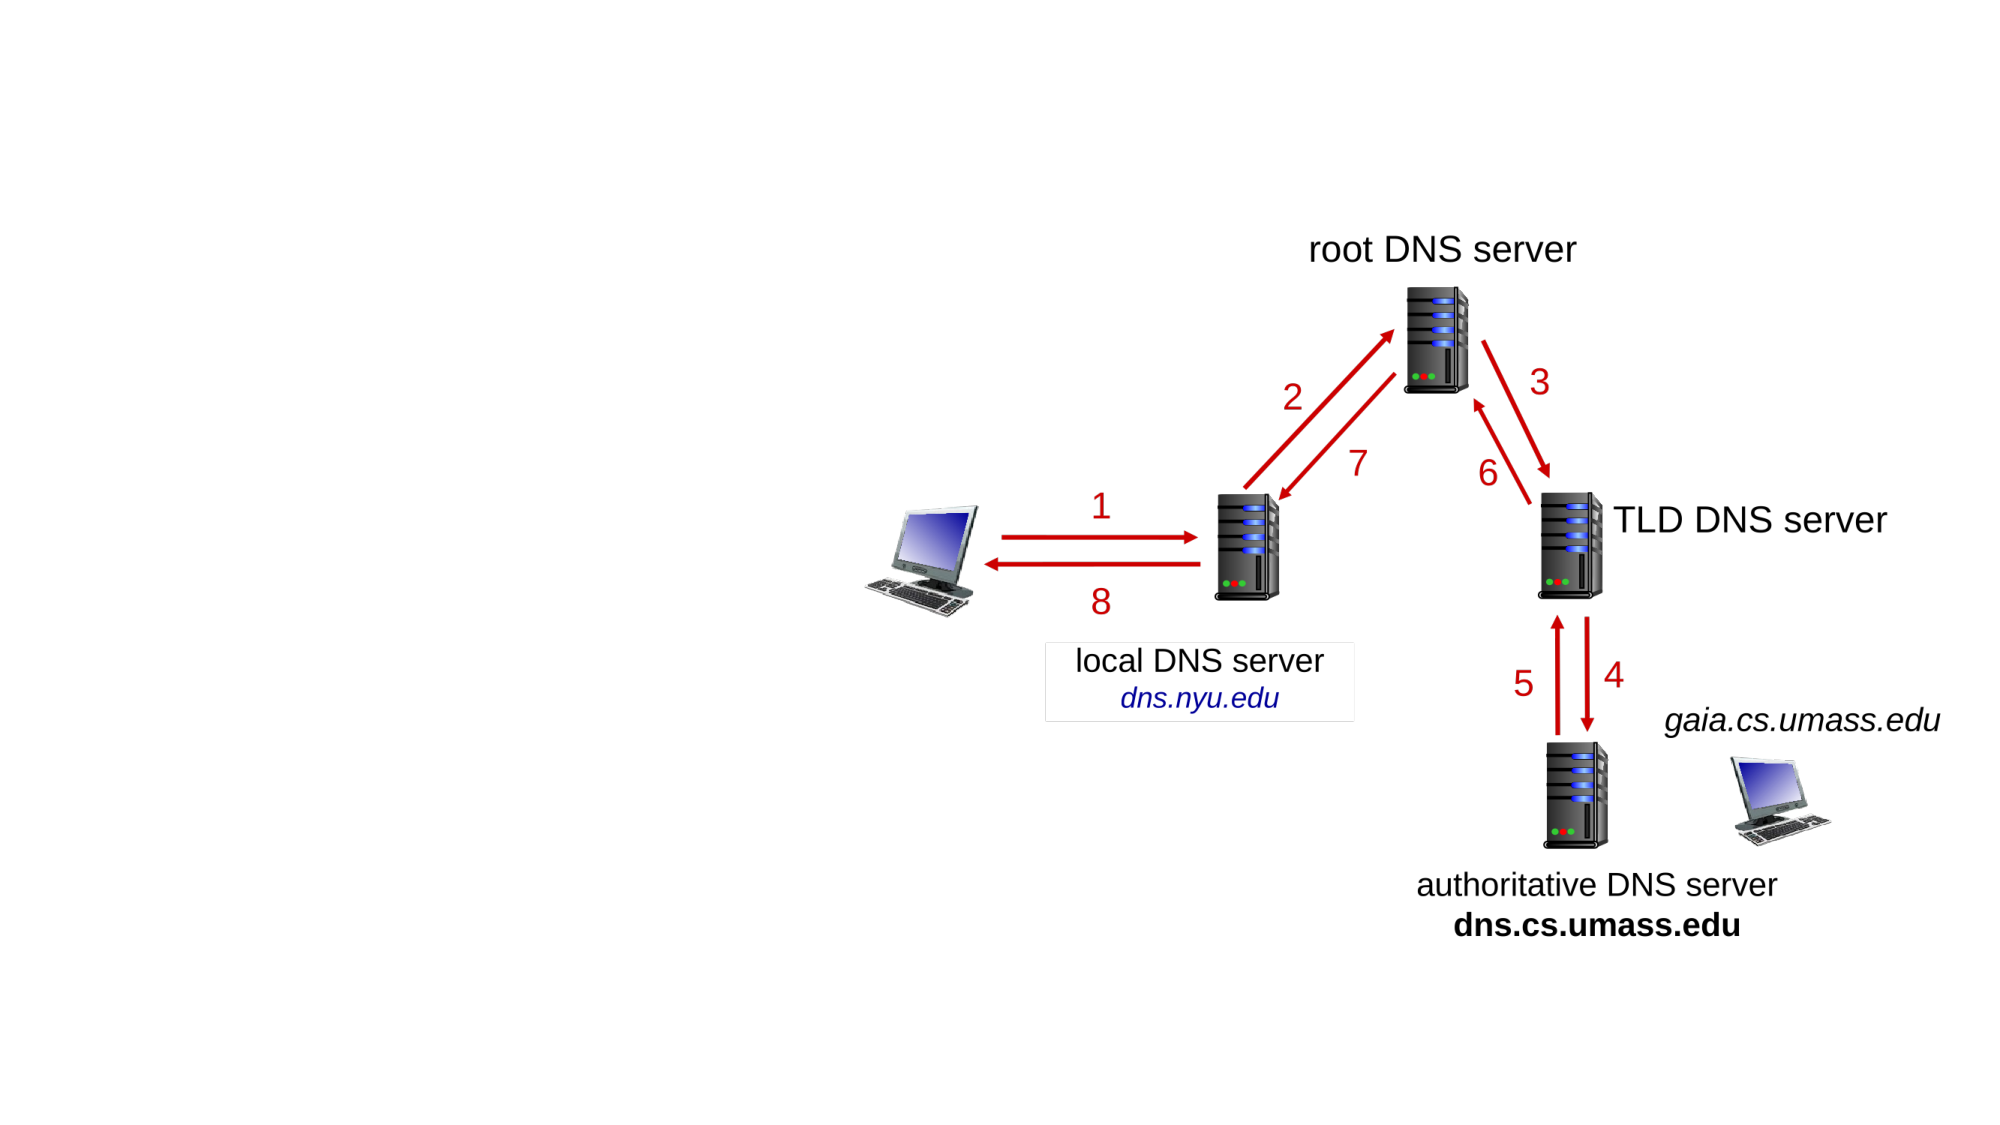
\includegraphics[width=4cm,trim={15cm 3cm 0 4cm},clip]{img/dns_recursive.pdf}    
      \end{center}
    \end{minipage}

\begin{minipage}{0.4\columnwidth}
    \begin{center}
\resizebox{0.9\textwidth}{!}{%
\rotatebox{90}{%
\rotatebox{270}{
    \hspace{-1cm}
    \texttt{uncached}\\
}
\begin{tabular}{|p{0.01\textwidth}|p{1.1\textwidth}|p{1.1\linewidth}|p{1.1\linewidth}|}

    \hline
     & Query to & src IP & dst IP \\
    \hline
    1  & www.tu-berlin.de & Client-IP & Local Resolver \\
    2  & .de NS & Local Resolver IP & root-DNS \\
    3  & .de NS Antwort & root-DNS & Local Resolver \\
    4  & tu-berlin.de NS & Local Resolver IP & .de DNS \\
    5  & tu-berlin.de NS Antwort & .de DNS & Local Resolver \\
    6  & www.tu-berlin.de A & Local Resolver IP & .tu-berlin DNS \\
    7  & www.tu-berlin.de A Antwort & .tu-berlin DNS & Local Resolver \\
    8  & www.tu-berlin.de IP & Local Resolver IP & Client-IP \\
    \hline
\end{tabular}
}
\rotatebox{90}{%
\rotatebox{270}{
    \hspace{-0.75cm}
    \texttt{cached}\\
}
\begin{tabular}{|p{0.01\textwidth}|p{1.1\textwidth}|p{1.1\linewidth}|p{1.1\linewidth}|}
    \hline
     & Query to & src IP & dst IP \\
    \hline
    1  & webmail.tu-berlin.de & Client-IP & Local Resolver \\
    2  & webmail.tu-berlin.de A & Local Resolver IP & .tu-berlin DNS \\
    3  & webmail.tu-berlin.de A Antwort & .tu-berlin DNS & Local Resolver \\
    4  & webmail.tu-berlin.de IP & Local Resolver IP & Client-IP \\
    \hline
\end{tabular}
}
}
    \end{center}
    \end{minipage}
\begin{minipage}{0.58\columnwidth}
      \begin{center}
\begin{tabular}{p{0.5\textwidth}|p{0.3\textwidth}}
local DNS-Server & everyone has one \\
\hline
Authoritative Name-Server  & accountbale for a specific host \\
\hline
Root Name-Server & 13 globally, per anycast \\
\end{tabular}
\vspace{0.1cm}
\hrule
\vspace{0.2cm}
\begin{tabular}{p{0.40\linewidth}p{0.50\linewidth}}
\verb!A! & Hostname, IPv4 \\
\verb!NS!  & for  Authoritative Name-Server \\
\verb!CNAME! & for aliases (CDNs) \\
\verb!MX! & Mail \\
\verb!AAAA! & IPv6 \\
\end{tabular}   
      \end{center}
    \end{minipage}



\hrule height 0.3mm 
\vspace{0.1cm}

\section{IP - Internet Protocol}
\textbf{IP Address}: Identifier for a host/router interface.
\begin{itemize}
            \setlength{\itemsep}{0pt}
    \item \textbf{IPv4}: 32-bit decimal
    \item \textbf{IPv6}: 128-bit hexadecimal
\end{itemize}

\subsection{Key Concepts}
\begin{itemize}
            \setlength{\itemsep}{0pt}
    \item \textbf{Interface}: Connects a host/router to a physical link.
    \item \textbf{Network}: Physical reachability without routers.
    \item \textbf{Link-local addresses}: Non-routable (e.g., \texttt{169.254.0.1/16}).
    \item \textbf{CIDR}: Divides network and host portions (e.g., \texttt{a.b.c.d/x}).
\end{itemize}

\subsection{Special Addresses}
\begin{itemize}
            \setlength{\itemsep}{0pt}
    \item IPv4: \texttt{127.0.0.0/8} (Loopback), \texttt{224.0.0.0/4} (Multicast), \texttt{10.0.0.0/8}, \texttt{192.168.0.0/16} (Private).
    \item IPv6: \texttt{::1/128} (Loopback), \texttt{2000::/3} (Global Unicast), \texttt{FC00::/7} (Private).
\end{itemize}

\subsection{Protocols}
\begin{itemize}
    \setlength{\itemsep}{0pt}
    \item \textbf{DHCP}: Dynamic IP assignment.
    \item \textbf{IPv6 SLAAC}: Stateless address configuration (router prefix, host ID).
    \item \textbf{NAT}:
        \begin{itemize}
            \setlength{\itemsep}{0pt}
            \item One \texttt{IP} for local devices, not directly addressable.
            \item \texttt{NAT Table}: Maps \texttt{WAN} and \texttt{LAN} addresses/ports.
        \end{itemize}
\end{itemize}

\texttt{NAT Table}\\
\begin{tabular}{|p{0.2\columnwidth}|p{0.2\columnwidth}|p{0.2\columnwidth}|p{0.1\columnwidth}|}
    \hline
    External Address & External Port & Internal Address & Internal Port \\
    \hline
\end{tabular}



\begin{tabular}{|p{0.1\linewidth}| p{0.25\linewidth}| p{0.2\linewidth} | p{0.2\linewidth}| }
\hline
\textbf{CIDR} & \textbf{Subnet mask} & \textbf{\# of IP addresses} & \textbf{\# of usable IP addresses} \\
\hline
/32 & 255.255.255.255 & 1 & 1 \\
/31 & 255.255.255.254 & 2 & 2* \\
/30 & 255.255.255.252 & 4 & 2 \\
/29 & 255.255.255.248 & 8 & 6 \\
/28 & 255.255.255.240 & 16 & 14 \\
/27 & 255.255.255.224 & 32 & 30 \\
/26 & 255.255.255.192 & 64 & 62 \\
/25 & 255.255.255.128 & 128 & 126 \\
/24 & 255.255.255.0 & 256 & 254 \\
/23 & 255.255.254.0 & 512 & 510 \\
/22 & 255.255.252.0 & 1,024 & 1,022 \\
/21 & 255.255.248.0 & 2,048 & 2,046 \\
/20 & 255.255.240.0 & 4,096 & 4,094 \\
/19 & 255.255.224.0 & 8,192 & 8,190 \\
/18 & 255.255.192.0 & 16,384 & 16,382 \\
/17 & 255.255.128.0 & 32,768 & 32,766 \\
/16 & 255.255.0.0 & 65,536 & 65,534 \\
/15 & 255.254.0.0 & 131,072 & 131,070 \\
/14 & 255.252.0.0 & 262,144 & 262,142 \\
/13 & 255.248.0.0 & 524,288 & 524,286 \\
/12 & 255.240.0.0 & 1,048,576 & 1,048,574 \\
/11 & 255.224.0.0 & 2,097,152 & 2,097,150 \\
/10 & 255.192.0.0 & 4,194,304 & 4,194,302 \\
/9 & 255.128.0.0 & 8,388,608 & 8,388,606 \\
/8 & 255.0.0.0 & 16,777,216 & 16,777,214 \\
/7 & 254.0.0.0 & 33,554,432 & 33,554,430 \\
/6 & 252.0.0.0 & 67,108,864 & 67,108,862 \\
/5 & 248.0.0.0 & 134,217,728 & 134,217,726 \\
/4 & 240.0.0.0 & 268,435,456 & 268,435,454 \\
/3 & 224.0.0.0 & 536,870,912 & 536,870,910 \\
/2 & 192.0.0.0 & 1,073,741,824 & 1,073,741,822 \\
/1 & 128.0.0.0 & 2,147,483,648 & 2,147,483,646 \\
/0 & 0.0.0.0 & 4,294,967,296 & 4,294,967,294 \\
\hline
\end{tabular}
\texttt{*often used for transfernets, f.e. two router}  




\hrule height 0.3mm 
\vspace{0.1cm}
\section{TCP - Transport Protocol}
\begin{tabular}{p{0.40\linewidth}p{0.50\linewidth}}
\verb!connection oriented, handshake before transmission! &  \\
\verb!point to point, reliable datastream!  &  \\
\verb!flow control and congestion control! & \\
\verb!mss - maximum segment size! & \\
\hline
\verb!Sequencenumber! & Byte Stream Nummer of the first 1 byte of the segmentdata \\
\verb!packet loss detect! & retransmission timeout or 3 double ACKs \\
\end{tabular}
\hrule
\textbf{Retransmission timeout - $T_{interval}$}
$RTT_{est,0} = RTT_{sample,0}$
\[
RTT_{est} = (1-\alpha)\cdot RTT_{est} + \alpha RTT_{sample}\text{, } \alpha=0.125
\]
\[
RTT_{dev} = (1-\beta)\cdot RTT_{dev} + \beta (|RTT_{sample}-RTT_{est}|)\text{, }\beta=0.25
\]
\[
T_{interval} = RTT_{est} + 4 \cdot RTT_{dev}
\]
Retransmitted Packets do not count into the RTT because, TCP does not not know if the ACK is from the original packet or the retransmitted.
\hrule
\vspace{1cm}
\textbf{Flow Control - FC} \\
\texttt{not overflow receiver's buffer} \\
\texttt{receiver informs sender about free buffer} \\
\texttt{sliding windows with size n, n bytes are sent} \\
\texttt{ideal } $w_{\text{size}} = \text{delay} \cdot \text{bandwidth} = \text{RTT} \cdot \text{bitrate}_{\text{bottleneck}}$
\hrule

\textbf{Congestion Control - CC} \\
\texttt{avoidance of lost packets (buffer overflow in router)} \\
\texttt{avoidance of long delays (queuing delays in router)}
\hrule

\textbf{Slowstart - SS} \\
\texttt{exponentially increase:} $2^{cwnd}$
\hrule

\textbf{Congestion Avoidance - CA} \\
\texttt{linear increase:} $cwnd++$
\hrule
\vspace{0.1cm}
\begin{tabular}{p{0.15\linewidth}|p{0.35\linewidth}p{0.35\linewidth}}
\textbf{} & \textbf{Timeout} & \textbf{3 additional Dup ACKs} \\
\hline
\textbf{Tahoe} & \[cwnd_n = 1\] \[ssthresh = \frac{cwnd_o}{2}\] and SS & \[cwnd_n = 1\] \[ssthresh = \frac{cwnd_o}{2}\] and SS \\
\hline
\textbf{Reno} & \[cwnd_n = 1\] \[ssthresh = \frac{cwnd_o}{2}\] and SS & \[cwnd_n = \frac{cwnd_o}{2}\] \[ssthresh = cwnd_n\] and CA \\
\end{tabular}
\texttt{Both start with $SS$ until $cwnd = ssthresh$ and then proceed doing $CA$ until} \textbf{Timeout} \texttt{or} \textbf{3 additional Dup ACKs}
\texttt{happen.}
if \textbf{3 additional Dup acks} are detected, the transmission round is is instantly stopped
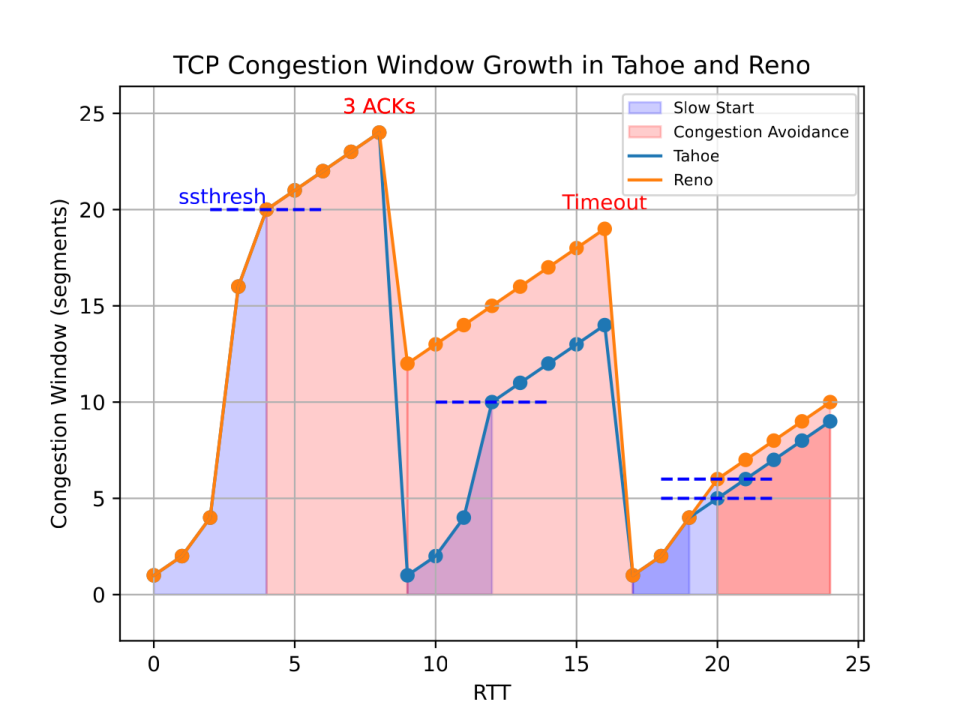
\includegraphics[width=\columnwidth]{img/tcp.pdf}
\hrule
\[
Throughput_{mean} = \frac{3}{4} \cdot \frac{cwnd [bytes]}{RTT[s]} [bytes/sec]
\] $cwnd$ where first loss occurs
\vspace{0.1cm}
\hrule
\resizebox{\columnwidth}{!}{%
    \rotatebox{90}{%
        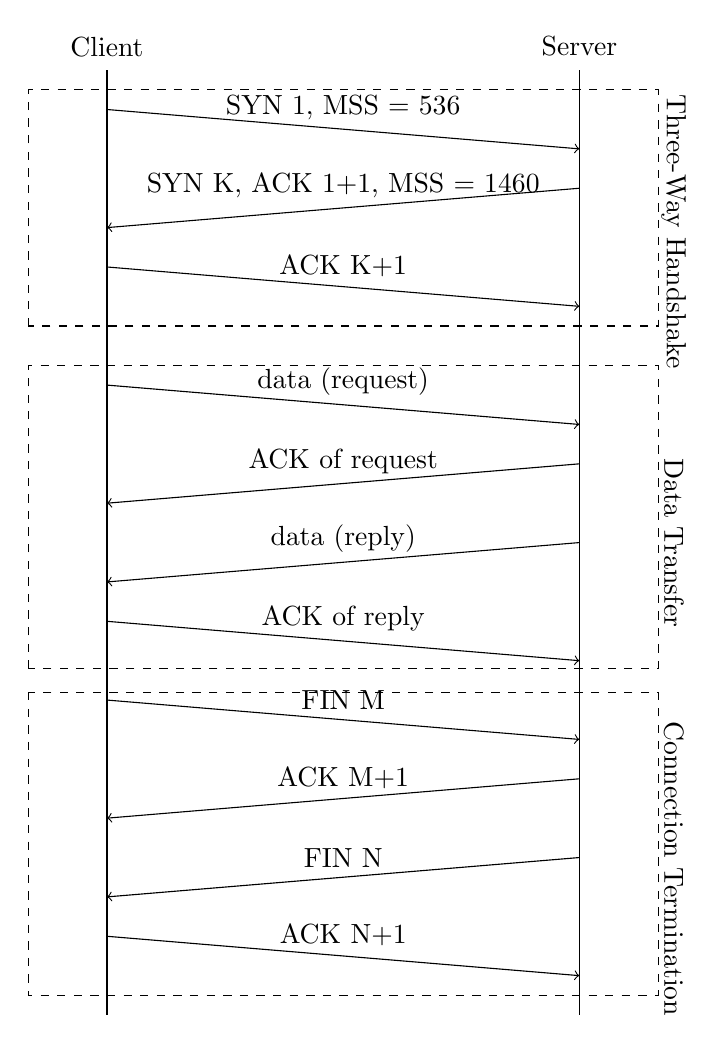
\begin{tikzpicture}
            % Drawing the vertical lines for Client and Server
            \draw (-3,0) -- (-3,-12) (3,0) -- (3,-12);
            
            % Labels for Client and Server
            \node at (-3,.3) {Client};
            \node at (3,.3) {Server};
            
            % Three-Way Handshake
            \draw[->] (-3,-0.5) -- node[midway,above] {SYN 1, MSS = 536} (3,-1);
            \draw[->] (3,-1.5) -- node[midway,above] {SYN K, ACK 1+1, MSS = 1460} (-3,-2);
            \draw[->] (-3,-2.5) -- node[midway,above] {ACK K+1} (3,-3);
            
            % Data Exchange
            \draw[->] (-3,-4) -- node[midway,above] {data (request)} (3,-4.5);
            \draw[->] (3,-5) -- node[midway,above] {ACK of request} (-3,-5.5);
            \draw[->] (3,-6) -- node[midway,above] {data (reply)} (-3,-6.5);
            \draw[->] (-3,-7) -- node[midway,above] {ACK of reply} (3,-7.5);
            
            % Connection Termination
            \draw[->] (-3,-8) -- node[midway,above] {FIN M} (3,-8.5);
            \draw[->] (3,-9) -- node[midway,above] {ACK M+1} (-3,-9.5);
            \draw[->] (3,-10) -- node[midway,above] {FIN N} (-3,-10.5);
            \draw[->] (-3,-11) -- node[midway,above] {ACK N+1} (3,-11.5);
            \draw[dashed] (-4,-3.25) rectangle (4,-0.25) 
            node[rotate=270, anchor=west, yshift=0.2cm, xshift=-2] {Three-Way Handshake};
        
            \draw[dashed] (-4,-7.6) rectangle (4,-3.75) 
            node[rotate=270, anchor=west, yshift=0.2cm, xshift=30] {Data Transfer};
        
            \draw[dashed] (-4,-7.9) rectangle (4,-11.75) 
            node[rotate=270, anchor=west, yshift=0.2cm, xshift=-102.5] {Connection Termination};
        \end{tikzpicture}
    }
}
\vspace{0.1cm}
\hrule height 0.3mm 

\section{UDP - Transport Protocol}
\texttt{besto effort}\\
\texttt{connection-less}\\
\texttt{can get lost, can arrive in different order}\\
\hrule
\textbf{Link Layer}
\textbf{Data Link Layer}:
    \begin{itemize}
            \setlength{\itemsep}{0pt}
            \item Error detection and correction.
            \item Broadcast channel: Multiple access.
            \item Link layer addressing.
            \item Half-duplex and full-duplex.
        \end{itemize}
    \textbf{MAC Protocols}:
        \begin{itemize}
            \setlength{\itemsep}{0pt}
            \item Channel partitioning (e.g., time, frequency).
            \item Random access: Handle collisions.
            \item Taking turns: Coordinate access to avoid collisions.
            \item Goal: Efficient, fair, simple, decentralized.
        \end{itemize}
\textbf{Addresses}:
        \vspace{0cm}
        \begin{itemize}
            \setlength{\itemsep}{0pt}
            \item \texttt{IP}: Network-layer addresses for routing.
            \item \texttt{MAC}: Data link-layer addresses for local communication.
            \item 48-bit \texttt{MAC} address: Embedded in NIC ROM.
        \end{itemize}
\textbf{Ethernet}:
        \begin{itemize}
            \setlength{\itemsep}{0pt}
            \item Dominant LAN technology.
            \item Uses \texttt{CSMA/CD}: Collision detection and handling.
            \item Exponential backoff: Wait time after collision.
            \item Kollision handling: Random delay on successive collisions.
        \end{itemize}
\textbf{ARP}:
    \begin{enumerate}
        \item A broadcasts an ARP query to FF:FF:FF:FF:FF:FF with B's IP.
        \item B replies with its MAC address (which is send to A).
        \item A updates its ARP table with the IP-to-MAC mapping and TTL.
    \end{enumerate}


\hrule height 0.3mm

\vspace{0.1cm}
\section{Routing}
\texttt{adressing, path determination with routing algos, switchting, forwarding}

\begin{itemize}
    \setlength{\itemsep}{0pt}  % No extra spacing
    \item \texttt{Global}: Full topology and link cost knowledge. (\texttt{Link-State})
    \item \texttt{Decentralized}: Knows only direct neighbors, iterative updates. (\texttt{Distance-Vector})
    \item \texttt{Static}: Routes change slowly over time.
    \item \texttt{Dynamic}: Routes update frequently via periodic updates or link cost changes.
\end{itemize}

\textbf{Intra-AS Routing}: Routing within an autonomous system.
\begin{itemize}
    \setlength{\itemsep}{0pt}
    \item \texttt{IGP}: Interior Gateway Protocols
    \item \texttt{RIP}: Routing Information Protocol
    \item \texttt{OSPF}: Open Shortest Path First (\texttt{Link-State Algorithm})
    \item \texttt{State}: Each router knows its reachable networks.
    \item \texttt{OSPF Advertisements}: Spread state info, database sync.
    \item \texttt{Link-State Database}: Stores all router states.
    \item \texttt{Hello Protocol}: Finds neighbors.
    \item \texttt{Hierarchical OSPF}: Used in large networks.
    \item \texttt{Router Hierarchy}:  
        \begin{itemize}
            \setlength{\itemsep}{0pt}
            \setlength{\itemsep}{0pt}
            \item 1 \texttt{Boundary Router}  
            \item \( n \) \texttt{Backbone Routers}  
            \item \( m \) \texttt{Area Border Routers}  
            \item Internal Routers  
        \end{itemize}
\end{itemize}

\textbf{Inter-AS Routing}: Routing between autonomous systems.
\begin{itemize}
    \setlength{\itemsep}{0pt}
    \item \texttt{BGP}: Border Gateway Protocol (de facto standard)
    \item \texttt{BGP Sessions}: BGP peers exchange routing info over semi-permanent TCP connections.
    \item \texttt{Path-Vector Protocol}: BGP tracks routes using AS paths.
    \item \texttt{AS-PATH}: Lists all ASs in a route.
    \item \texttt{NEXT-HOP}: Internal AS router to the next-hop AS.
    \item \texttt{Route}: Defined by prefix + attributes.
    \item \texttt{Ingress Filtering}: Gateway router validates/filters route proposals (e.g., to prevent loops).
    \item \texttt{Routing Policy}: Aligned with provider goals (cost efficiency).
    \item \texttt{Local Preference}: Routes with the highest preference are favored.
    \item \textbf{Route Selection Criteria}:  
        \begin{itemize}
            \setlength{\itemsep}{0pt}
            \item Highest \texttt{Local Preference}
            \item Shortest \texttt{AS-PATH}
            \item Best \texttt{MED} (Multi-Exit Discriminator)
            \item Nearest \texttt{NEXT-HOP} (Hot Potato Routing)
            \item Peer’s IP Address
        \end{itemize}
\end{itemize}
\begin{tabular}{|p{0.16\columnwidth}|p{0.1\columnwidth}|p{0.1\columnwidth}|p{0.12\columnwidth}|p{0.1\columnwidth}|p{0.1\columnwidth}|}
\hline
\textbf{}               & {\tiny Own Routes} & {\tiny Customers Routes} & {\tiny Siblings Routes} & {\tiny Providers Route} & {\tiny Peers Route} \\ \hline
Advertising to Provider & yes                 & yes                       & yes                      &                          &             \\ \hline
Advertising to Customer & yes                 & yes                       & yes                      & yes                      & yes         \\ \hline
Advertising to Peer     & yes                 & yes                       & yes                      &                          &             \\ \hline
\end{tabular}
\vspace{0.1cm}
\hrule height 0.3mm 
\vspace{0.1cm}

\textbf{Hard State vs. Soft State}  
\begin{itemize}
    \setlength{\itemsep}{0pt}
    \item \textbf{Hard State}:  
        \begin{itemize}
            \setlength{\itemsep}{0pt}
            \item Installed during connection setup, removed upon termination (e.g., TCP, SS7).
            \item Assumption: State remains valid until explicitly changed.
            \item Reliable signaling with explicit state deletion.
            \item Inconsistency and overhead decrease with state lifetime.
            \item Explicit removal improves consistency with minimal overhead.
        \end{itemize}
    \item \textbf{Soft State}:  
        \begin{itemize}
                \setlength{\itemsep}{0pt}
            \item Installed during connection setup, maintained via refresh messages, removed by timeout or lack of refresh (e.g., RSVP, IGMPv1).
            \item Assumption: State becomes invalid if not refreshed.
            \item Uses a refresh timer at sender and a timeout timer at receiver.
            \item Easier fault detection, only implicit reliability.
        \end{itemize}
\end{itemize}

\hrule height 0.3mm 
\vspace{0.1cm}
\textbf{Internet Signaling}  

\begin{itemize}
    \setlength{\itemsep}{0pt}
    \item \textbf{In-Band Signaling}:  
        \begin{itemize}
            \setlength{\itemsep}{0pt}
            \item \texttt{HTTP}: Messages combine signaling and data.  
            \item \texttt{SIP (Session Initiation Protocol)}: Uses the same channel for control and media setup.  
            \item \texttt{Telnet}: Commands and data are sent over the same connection.  
        \end{itemize}
    \item \textbf{Out-of-Band Signaling}:  
        \begin{itemize}
            \setlength{\itemsep}{0pt}
            \item \texttt{FTP}: Uses a dedicated control connection.  
            \item \texttt{H.323}: Control and media streams use separate channels.  
            \item \texttt{SS7}: Uses a separate network for signaling in telecom systems.  
        \end{itemize}
\end{itemize}


\hrule height 0.3mm 

\begin{tabular}{p{0.40\linewidth}p{0.50\linewidth}}
\verb!packet switched! & logical connection, via multipath  \\
\verb!circuit switched!  & static connection for the whole communication, resources are allocated for the whole connection lifespan \\
\end{tabular}
\texttt{Number of Users for CS:}\\
\(
\#user = \frac{Bandwidth_{all} [\frac{mbit}{s}]}{Bandwdith_{user}[\frac{mbit}{s}]}
\)\\
    \begin{minipage}{0.4\columnwidth}
    \begin{center}
    \textbf{Packet Switched}
      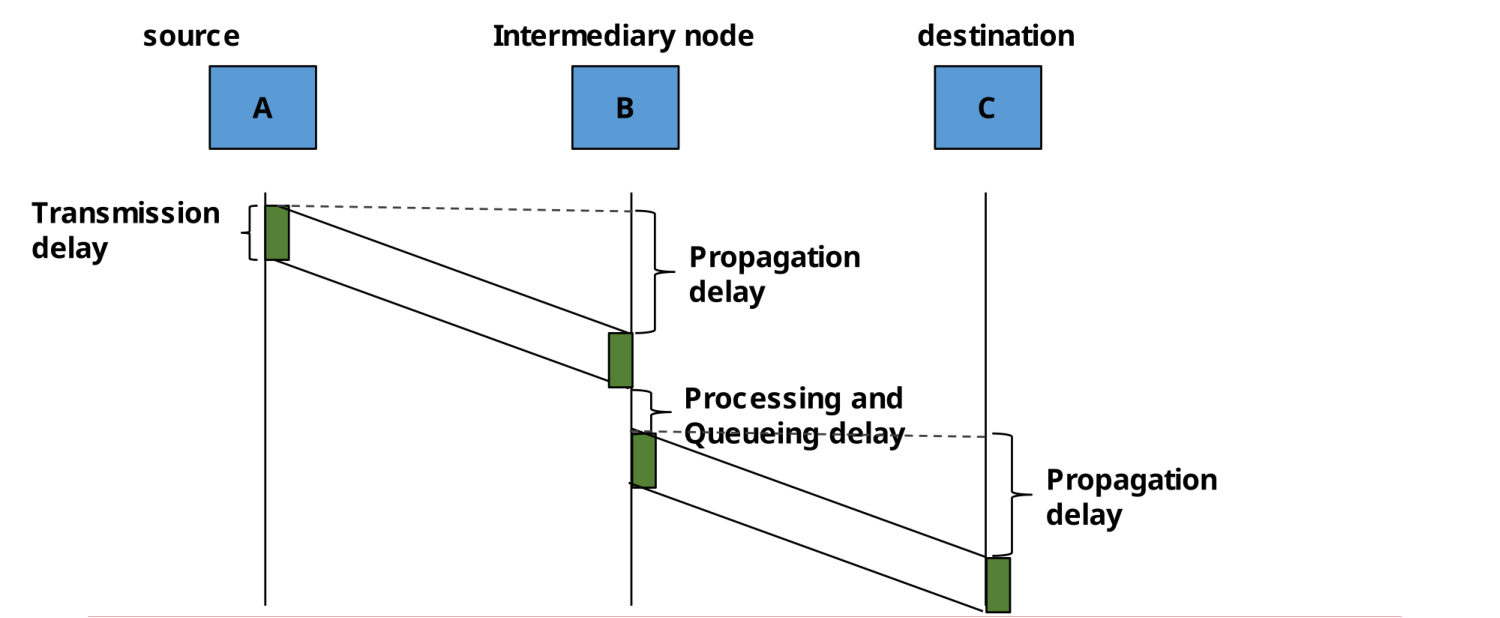
\includegraphics[width=5cm]{img/ps_delay.pdf}  
    \end{center}
    \end{minipage}
    \begin{minipage}{0.48\columnwidth}
      \begin{center}
        \textbf{Circuit Switched}
        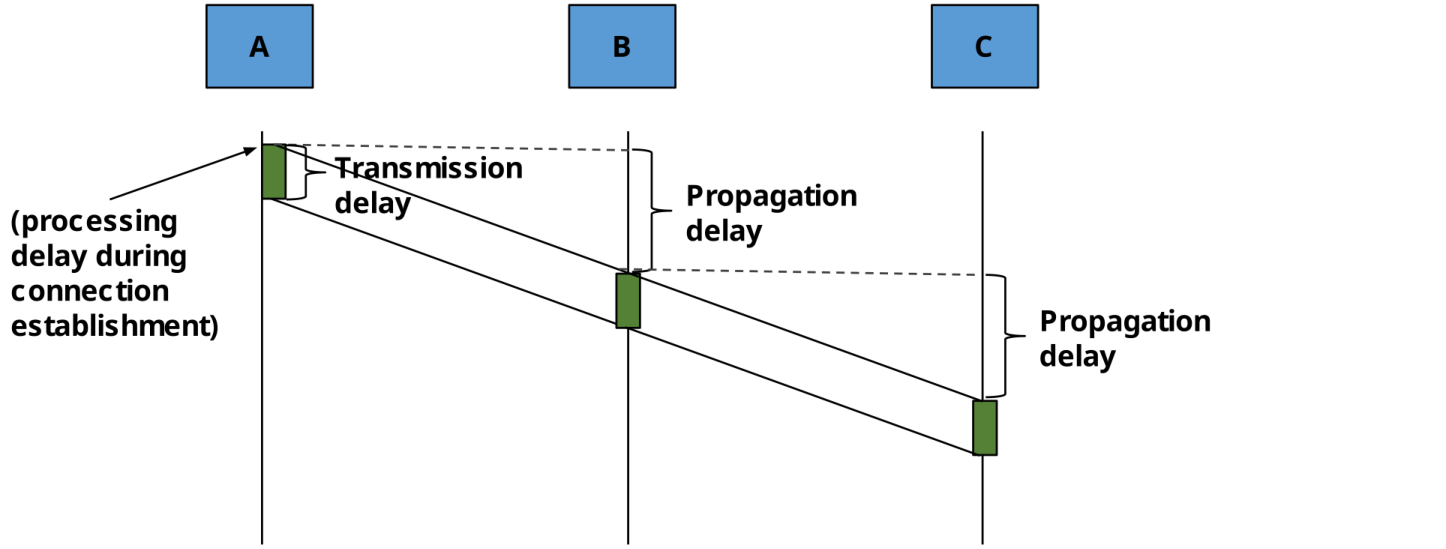
\includegraphics[width=5cm]{img/cs_delay.pdf}    
      \end{center}
    \end{minipage}
\hrule
    \textbf{Types of Network Delays}:  
        \begin{itemize}
            \setlength{\itemsep}{0pt}
            \item \texttt{Transmission Delay}: Time required to push all bits of a packet onto the wire. 
            \item \texttt{Propagation Delay}: Time for a bit to travel through the link, depending on the physical medium.  
            \item \texttt{Processing Delay}: Time needed to inspect the packet header and determine its forwarding path.  
            \item \texttt{Queuing Delay}: Time a packet spends waiting in the queue before transmission, influenced by queue length.  
        \end{itemize}
\hrule height 0.3mm 
        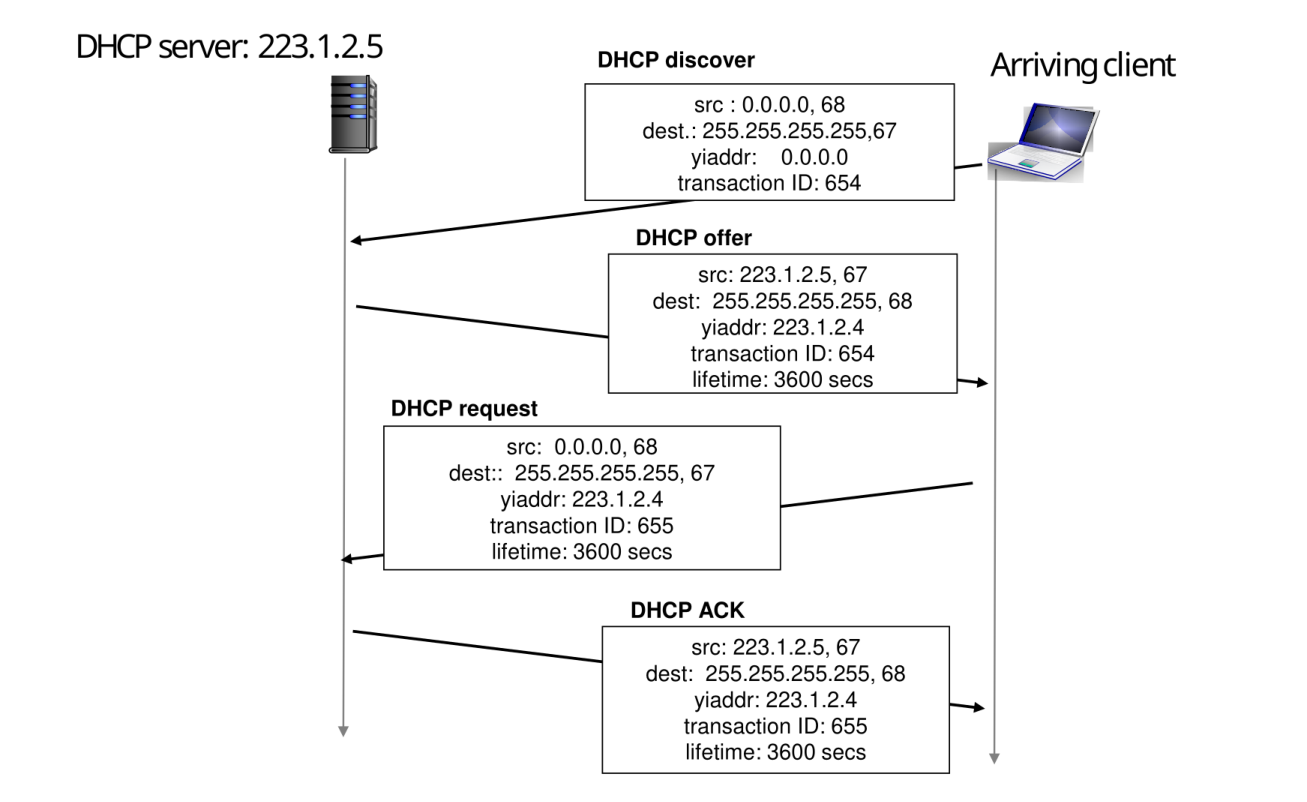
\includegraphics[width=\columnwidth]{img/dhcp.pdf}
\hrule height 0.3mm

\texttt{Forwarding Table}
\begin{tabular}{|l|l|l|}
    \hline
    Prefix & Next Hop & Interface \\
    \hline
    192.168.1.0/24 & 10.0.0.1 & eth0 \\
    10.0.0.0/8 & 192.168.1.1 & eth1 \\
    172.16.0.0/16 & 10.0.0.2 & eth2 \\
    \hline
\end{tabular}

\hrule height 0.3mm
\texttt{if all network caches are empty:}\\
\begin{enumerate}
    \setlength{\itemsep}{0pt}
    \item \texttt{ARP}
    \item \texttt{DNS} 
    \item \texttt{IP}
    \item \texttt{TCP/UDP}
\end{enumerate}
\hrule height 0.3mm
    \begin{minipage}{0.49\columnwidth}


\rotatebox{90}{%
    \parbox{5cm}{ % Adjust width as needed
        \centering
        \textbf{Delay Types} \\[0.5em]
        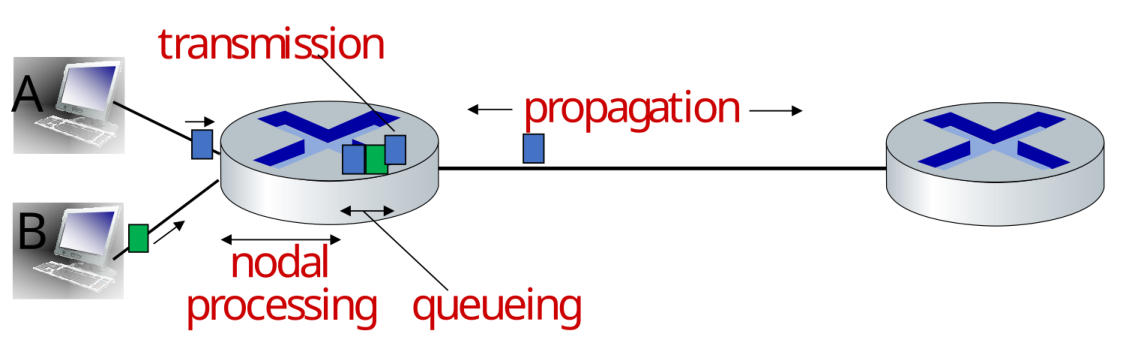
\includegraphics[width=7cm]{img/delay.pdf} \\[0.5em]
        \[
        d_{\text{nodal}} = d_{\text{proc}} + d_{\text{queue}} + d_{\text{trans}} + d_{\text{prop}}
        \]
    }
}
    \end{minipage}
    \begin{minipage}{0.49\columnwidth}
    $d_{proc}$: nodal processing
    \begin{itemize}
        \item check bit errors
        \item determine output link
        \item typically <msec
    \end{itemize}
    $d_{queue}$: queueing delay
    \begin{itemize}
        \item time waiting at output link for transmission
        \item depends on congestion level of router
    \end{itemize}
    $d_{trans}$: transmission delay
    \begin{itemize}
        \item $L$ packet lengths [bits]
        \item $R$ link transmission rate [bps]
    \end{itemize}
    $d_{trans}$ = $\frac{L}{R}$\\
    $d_{prop}$: propagation delay
    \begin{itemize}
        \item $d$ length of physical link $[m]$
        \item $s$ propagation speed $2\cdot10^8 [m/s]$
    \end{itemize}
    $d_{pop}=d/s$
    \end{minipage}
\hrule height 0.3mm

    \begin{tabular}{|l|c|r|}
        \hline
        \textbf{Prefix} & \textbf{Symbol} & \textbf{Power of 10} \\
        \hline
        Tera  & T  & $10^{12}$ \\
        Giga  & G  & $10^{9}$  \\
        Mega  & M  & $10^{6}$  \\
        Kilo  & k  & $10^{3}$  \\
        Hecto & h  & $10^{2}$  \\
        Deca  & da & $10^{1}$  \\
        Base Unit & - & $10^{0}$  \\
        Deci  & d  & $10^{-1}$  \\
        Centi & c  & $10^{-2}$  \\
        Milli & m  & $10^{-3}$  \\
        Micro & $\mu$  & $10^{-6}$  \\
        Nano  & n  & $10^{-9}$  \\
        \hline
    \end{tabular}
\hrule height 0.3mm

Switches break collision domain but not broadcast domains. Router break collision domain and broadcast domain.
Hubs break nothing.

\hrule height 0.3mm
    \rotatebox{90}{%
\[
\begin{array}{|c|c|c|c|}
\hline
0x00 & 0x01 & 0x02 & 0x03 \\
\hline
0x04 & 0x05 & 0x06 & 0x07 \\
\hline
0x08 & 0x09 & 0x0A & 0x0B \\
\hline
0x0C & 0x0D & 0x0E & 0x0F \\
\hline
0x10 & 0x11 & 0x12 & 0x13 \\
\hline
0x14 & 0x15 & 0x16 & 0x17 \\
\hline
0x18 & 0x19 & 0x1A & 0x1B \\
\hline
0x1C & 0x1D & 0x1E & 0x1F \\
\hline
0x20 & 0x21 & 0x22 & 0x23 \\
\hline
0x24 & 0x25 & 0x26 & 0x27 \\
\hline
0x28 & 0x29 & 0x2A & 0x2B \\
\hline
0x2C & 0x2D & 0x2E & 0x2F \\
\hline
0x30 & 0x31 & 0x32 & 0x33 \\
\hline
0x34 & 0x35 & 0x36 & 0x37 \\
\hline
0x38 & 0x39 & 0x3A & 0x3B \\
\hline
0x3C & 0x3D & 0x3E & 0x3F \\
\hline
\end{array}
\]
}
\hrule height 0.3mm

$\text{Bytes} = \frac{\text{Bits}}{8}$,
$\text{Bits} = \text{Bytes} \cdot 8$
\hrule height 0.3mm
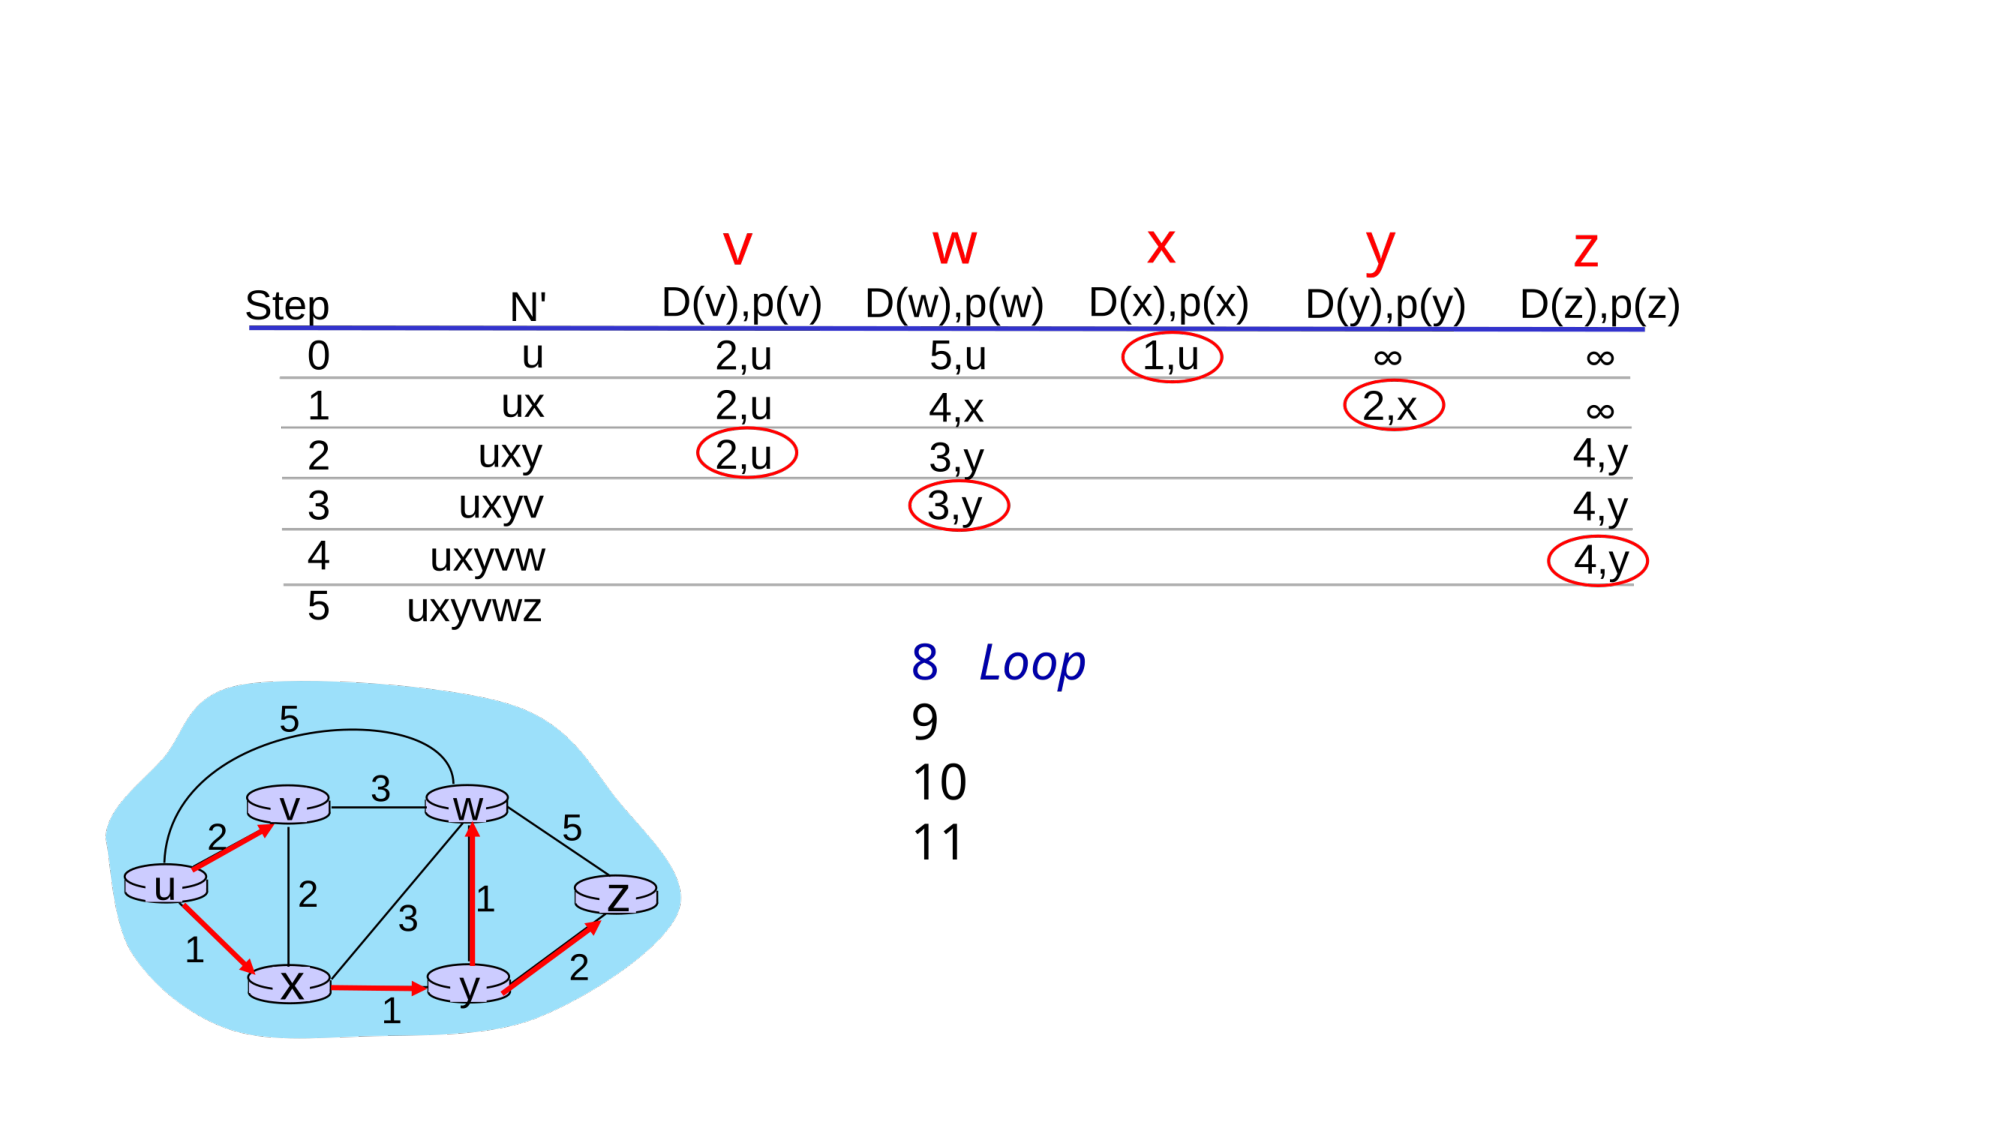
\includegraphics[width=\columnwidth]{img/djkstra.pdf}
\hrule height 0.3mm
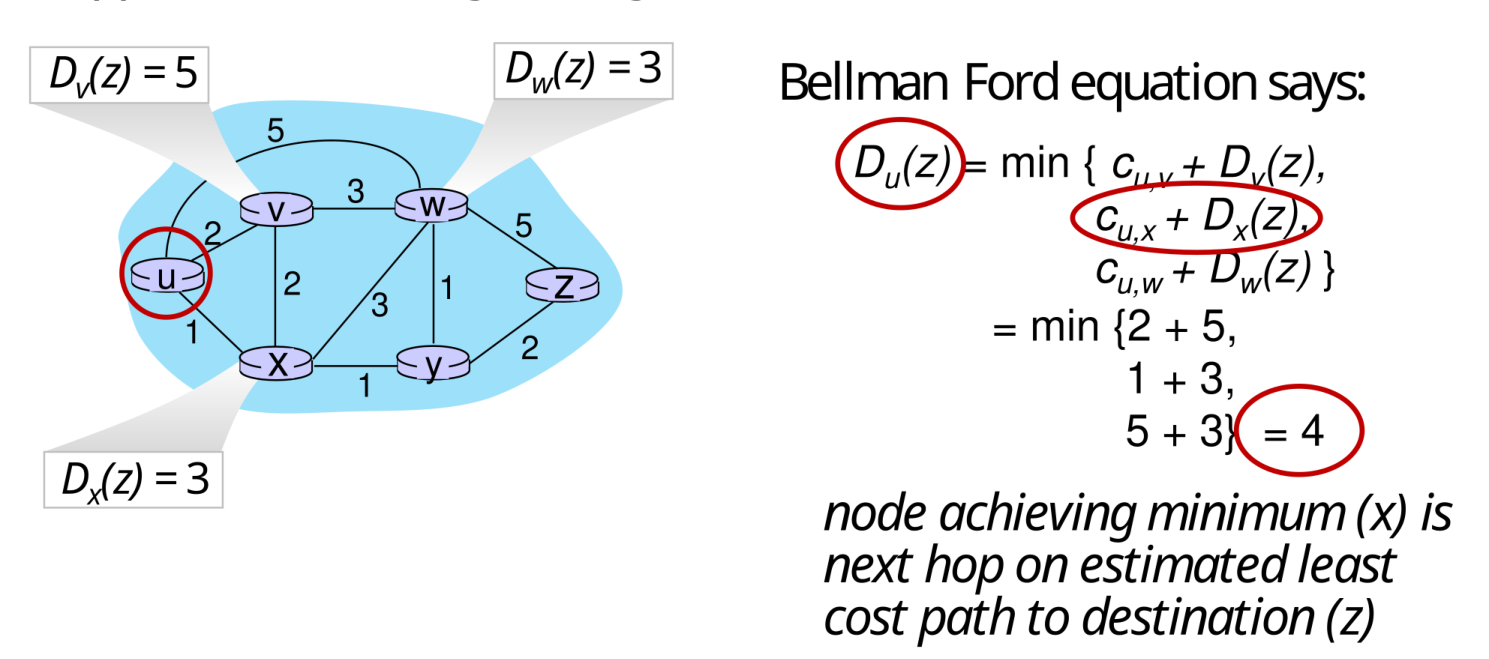
\includegraphics[width=\columnwidth]{img/bellmann.pdf}
\hrule height 0.3mm
\begin{enumerate}
    \item \textbf{Omit leading zeros:} Remove leading zeros in each 16-bit segment.
    \item \textbf{Use double colons (::) for consecutive zeros:} Replace the longest contiguous sequence of all-zero segments with \texttt{::}. This can be done only once in an address.
    \item \textbf{Do not shorten single zeros unnecessarily:} If there are multiple zero sequences of the same length, replace only the first one to avoid ambiguity.
\end{enumerate}

\section{Example}
Consider the following IPv6 address:

\begin{verbatim}
2001:0db8:0000:0000:0000:ff00:0042:8329
\end{verbatim}

Applying the rules:

\begin{enumerate}
    \item Remove leading zeros in each segment:
    
    \begin{verbatim}
    2001:db8:0:0:0:ff00:42:8329
    \end{verbatim}

    \item Replace the longest sequence of consecutive zeros with \texttt{::}:
    
    \begin{verbatim}
    2001:db8::ff00:42:8329
    \end{verbatim}
\end{enumerate}

Thus, the shortened IPv6 address is:

\begin{verbatim}
2001:db8::ff00:42:8329
\end{verbatim}
\hrule height 0.3mm
\end{multicols}
\end{document}